\documentclass{article}
\usepackage{amsmath}
\usepackage{hyperref}
\usepackage{tikz}
\usetikzlibrary{calc,arrows,shapes,positioning}
\usepackage{tkz-euclide}
\usepackage[numbib]{tocbibind}
\usepackage{float}
\usepackage{array}

\begin{document}

% Tikz code used to support block diagrams
% credit: https://tex.stackexchange.com/questions/175969/block-diagrams-using-tikz

\tikzset{
block/.style = {draw, fill=white, rectangle, minimum height=3em, minimum width=3em},
tmp/.style  = {coordinate}, 
circ/.style= {draw, fill=white, circle, node distance=1cm, minimum size=0.6cm},
input/.style = {coordinate},
output/.style= {coordinate},
pinstyle/.style = {pin edge={to-,thin,black}}
}

\title{An Autoencoder for Transmission of Vocoder Features over Radio Channels}
\maketitle

\section{Introduction}

This report presents an autoencoder derived from RDOVAE \cite{valin2023lowbitrate} to send speech over radio channels.  Our goal is to determine if reasonable speech quality can be obtained over a channel of bandwidth $B<3000$ Hz and SNR around 0dB, roughly the lower limit of Single Side Band (SSB) - a popular power and bandwidth efficient form of speech communication.

This document describes the Radio Autoencoder \emph{radae} system, discusses channels simulation and calibration, and describes how we combined ML with classical DSP to create a practical proof of concept system that can send speech over real world VHF and HF radio channels.  Finally, we compare the capabilities of the Radio Autoencoder to existing systems for speech communication over HF and VHF/UHF radio.

\begin{figure}[h]
\caption{Radio Autoencoder Concept}
\label{fig:radae_block}
\begin{center}
\begin{tikzpicture}[auto, node distance=2cm,>=triangle 45,x=1.0cm,y=1.0cm,align=center,text width=1.5cm]

\node [input] (rinput) {};
\node [input, right of=rinput,node distance=0.5cm] (z) {};
\node [block, right of=z, node distance=1.5cm,text width=2cm] (feature_ext) {Feature Extraction};
\node [block, below of=feature_ext,node distance=2cm] (radae_enc) {\emph{radae} Encoder};
\node [block, right of=radae_enc,node distance=2.5cm] (channel) {Radio Channel};
\node [block, right of=channel,node distance=2.5cm] (radae_dec) {\emph{radae} Decoder};
\node [block, below of=radae_dec,node distance=2cm] (fargan) {\scalebox{0.8}[0.8]{FARGAN}};
\node [output, right of=fargan,node distance=2cm] (routput) {};

\draw [->] node[align=left,text width=2cm] {Input Speech} (rinput) -- (feature_ext);
\draw [->] (feature_ext) -- node[left, text width=0.5cm] {$\bf{f}$} (radae_enc);
\draw [->] (radae_enc) -- node[above, text width=0.5cm] {$\bf{z}$} (channel);
\draw [->] (channel) -- node[above, text width=0.5cm] {$\hat{\bf{z}}$} (radae_dec);
\draw [->] (radae_dec) -- node[left, text width=0.5cm] {$\hat{\bf{f}}$} (fargan);
\draw [->] (fargan) -- (routput) node[right, align=left, text width=1.5cm] {Output Speech};

\end{tikzpicture}
\end{center}
\end{figure}

The encoder (Figure \ref{fig:radae_block}) takes as input a typical set of vocoder features (short term spectrum, pitch, voicing), then applies time based prediction and transforms to produce a set of parameters that can be sent over a channel. This is similar to vocoders using classical DSP, except Machine Learning (ML) allows us to learn non-linear transforms and prediction, which tend to be more powerful.

In conventional digital speech systems, after the transformation/prediction stage we then quantise to a low bit rate, then use Forward Error  Correction (FEC) and modems to send the bits over a channel. However our work takes a novel twist – we train the autoencoder to generate PSK symbols that we send over the channel. It effectively combines quantisation, channel coding, and modulation. The symbols from the autoencoder tend to cluster around +/-1 like BPSK but are continuously valued, so can be considered discrete time, continuously valued PSK.

The encoder and decoder are trained together as an autoencoder with the loss function  $L(\bf{f},\hat{\bf{f}})$ applied to the vocoder features.  We employ the \scalebox{0.8}[0.8]{FARGAN} vocoder for speech analysis and synthesis, however the concept is applicable to any neural and even classical vocoder with a similar feature set.

Given a vector of vocoder features $\bf{f}$, we use an encoder to map them to a dimension $d$ latent vector $\bf{z}$ where $d$ is even.  Unlike digital modulation, each element $z_i$ of $\bf{z}$ is continuously valued and not constrained to a discrete set of points.  For bandwidth efficient transmission over the channel the elements of $\bf{z}$ are mapped to $d/2$ complex symbols $\bf{q}$. Compared to classical digital modulation, the elements of $\bf{z}$ can be considered BPSK symbols (continuously valued, analog bits), and the elements of $\bf{q}$ analog QPSK symbols.

\section{Simulation of AWGN Channels}

The autoencoder output $\bf{z}$ is updated every $T_z=1/R_z$ seconds, giving a BPSK symbol rate of:
\begin{equation}
R_b=d/T_z
\end{equation}
For example with $T_z=0.04, d=80, R_b=2000$ symbols/s.  The QPSK symbol rate is given by:
\begin{equation}
R_q = \frac{d}{2T_z} 
\end{equation}
For example with $T_z=0.04, d=80, R_q=1000$ symbols/s.

\begin{figure}[H]
\caption{Real sampled off-air signal.  We are interested in the blue bandpass interval of bandwidth $B$, which is single sided and hence complex valued. After shifting to baseband, it's power is unchanged, and it remains complex valued.}
\vspace{5mm}
\label{fig:bandpass}
\begin{center}
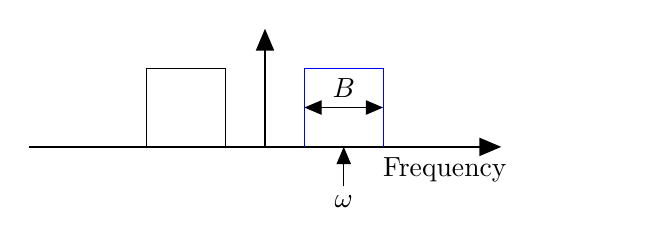
\begin{tikzpicture}[>=triangle 45,x=1.0cm,y=1.0cm]
\draw[thick,->] (-3,0) -- (3,0) node [below, align=left, text width=3cm]{Frequency};
\draw[thick,->] (0,0) -- (0,1.5);
\draw (-1.5,0) -- (-1.5,1) -- (-0.5,1) -- (-0.5,0);
\draw[blue] (0.5,0) -- (0.5,1) -- (1.5,1) -- (1.5,0);
\draw[<->] (0.5,0.5) -- node [above]{$B$}(1.5,0.5); 
\draw[->] (1,-0.5)  node [below]{$\omega$} -- (1,0);
\end{tikzpicture}
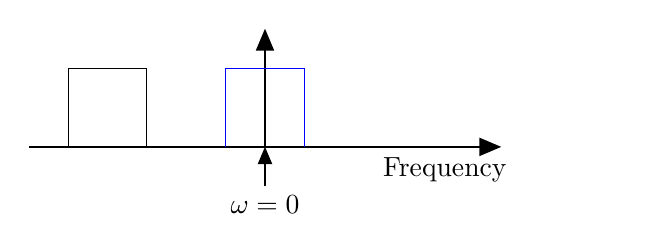
\begin{tikzpicture}[>=triangle 45,x=1.0cm,y=1.0cm]
\draw[thick,->] (-3,0) -- (3,0) node [below, align=left, text width=3cm]{Frequency};
\draw[thick,->] (0,0) -- (0,1.5);
\draw (-2.5,0) -- (-2.5,1) -- (-1.5,1.0) -- (-1.5,0);
\draw[blue] (-0.5,0) -- (-0.5,1) -- (0.5,1) -- (0.5,0);
\draw[->] (0,-0.5)  node [below]{$\omega=0$} -- (0,0);
\end{tikzpicture}
\end{center}
\end{figure}

We wish to simulate an AWGN channel with a user-defined $E_b/N_0$, where $E_b$ is the energy of each BPSK symbol, and $N_0$ is the noise power per unit bandwidth.  Consider a real valued signal sampled off air (Figure \ref{fig:bandpass}).  We will follow convention and define signal and noise power in the ``single sided" bandpass interval of the frequency spectrum with bandwidth B centred on $\omega$.  As the interval is single sided, we must use complex valued quantities to represent it.

We wish to simulate a bandpass AWGN channel at baseband ($\omega=0$).  This implies a frequency shift of the complex valued signal, but the signal remains complex valued and it's power is unchanged. The negative frequency component on the LHS of Figure \ref{fig:bandpass} is redundant and after frequency shifting can be removed by filtering.

Note that even at baseband we must use complex valued quantities for the signal and noise to represent a bandpass signal of bandwidth $B$.  As a counter-example, given a fixed sample rate $B$ and noise power $N$, a real valued noise sequence can only represent a bandwidth of $B/2$ which results in doubling the noise density $N_0=N/(B/2)=2N_0$ compared to a complex valued noise sequence with the same power.   

The energy of each BPSK symbol $E_b$ is the signal power $S$ divided by the symbol rate $R_b=1/T_b$.  The noise per unit bandwidth is the total noise power $N$ divided by the bandwidth $B$ of the system.  If we are simulating at one sample per symbol, $B=R_b$:
\begin{equation}
\begin{split}
\frac{E_b}{N_0} &= \frac{S/R_b}{N/R_b} \\
                &= \frac{S}{N} \\
                &= \frac{A^2}{\sigma^2}
\end{split}
\end{equation}
where $A$ is the amplitude of each BPSK symbol and $\sigma^2=N$ is the variance of the complex valued noise (mean noise energy per sample).  Given a set point $E_b/N_0$:
\begin{equation}
\label{eq:noise_sigma}
\sigma = \frac{A}{\sqrt{E_b/N_0}}
\end{equation}
The complex noise sample $r_i$ can be generated as:
\begin{equation}
r_i = \frac{\sigma}{\sqrt{2}}(\mathcal{N}_{2i}(0,1) + j\mathcal{N}_{2i+1}(0,1))
\end{equation}
where $\mathcal{N}_i(0,1)$ is the $i-th$ sample of a unit variance, zero mean, real Gaussian noise source.  Note the noise power is split evenly between the real and imaginary arms. Our symbols passing through an AWGN channel can be simulated at complex baseband as:
\begin{equation}
\begin{split}
\hat{z}_i &= z_i + r_i \\
\hat{q}_i &= q_i + r_i
\end{split}
\end{equation}
If the noise is zero mean, we can estimate $\sigma^2$ over $K$ noise samples $r_i$ as:
\begin{equation}
\sigma^2 = E[|r_i|^2] = \frac{1}{K}\sum_{i=0}^{K-1}|r_i|^2 
\end{equation}

\subsection{SNR Measurement}

In order to compare with other methods of speech communication that have varying bandwidths $B$, it is useful to formulate expressions for estimating SNR from the BPSK and QPSK symbols.  The Signal to Noise ratio (SNR) is given by:
\begin{equation}
\label{eq:snr_theory}
\begin{split}
\frac{S}{N} &= \frac{E_bR_b}{N_0B} \\
            &= \frac{E_qR_q}{N_0B}
\end{split}
\end{equation}
A noise bandwidth $B$ needs to be selected; common choices are $B=R_b$, in which case $S/N=E_b/N_0$; for HF radio $B=3000$ Hz to compare with existing analog and digital voice waveforms; or $B=1$ to obtain a normalised $C/N_0$ carrier power to noise density ratio - useful for comparing waveforms with different bandwidths.
 
At one sample per symbol, the power, the mean energy of each QPSK symbol over a window of $K$ samples is given by:
\begin{equation}
E_q = E[|q_i|^2] = \frac{1}{K}\sum_{i=0}^{K-1}|q_i|^2
\end{equation}
Note the variance function should not be used to calculate $E_q$, as we cannot guarantee $q_i$ is zero mean. As each QPSK symbol contains 2 BPSK symbols, the energy is split evenly:
\begin{equation}
\label{eq:Eb_Es}
E_b = E_q/2
\end{equation}
For example if the symbol amplitude is $A=1, E_b=A^2=1$, then $E_q=1+1=2$.

For transmission over multipath channels using OFDM we arrange the QPSK symbols as $N_c$ parallel carriers, each running at a symbol rate of $R_s=R_q/N_c$ symbols/s, where $R_s$ is chosen based on delay spread considerations.  Typical values for HF modems are $N_c=20$ and $R_s=50$ Hz. However the OFDM carriers are arranged such that the total symbol rate over the channel remains constant.  So for a given signal power $E_q$ and $E_b$ remain constant (Table \ref{tab:constant_eb}).

\begin{table} [H]
\centering
\begin{tabular}{l l l l l l l}
 \hline
 Waveform            & $N_c$ & $R_s$ & $R_q$ & $R_b$ & $E_q$ & $E_b$ \\
 \hline
 Single Carrier BPSK & 1     & -  & -    & 2000  & -        & $S/2000$ \\
 Single Carrier QPSK & 1     & -  & 1000 & 2000  & $S/1000$ & $S/2000$ \\
 OFDM QPSK           & 20    & 50 & 1000 & 2000  & $S/1000$ & $S/2000$ \\
 \hline
\end{tabular}
\caption{$E_b$ and $E_q$ examples for single and multi-carrier OFDM waveforms for constant carrier power $S$}
\label{tab:constant_eb}
\end{table}

\subsection{Calibration and Testing}

In order to evaluate the ML system early in the development process it is important to ensure the noise is correctly calibrated. The expressions above can be used to check the noise injection process:
\begin{enumerate}
\item Set a target $E_b/N_0$ for the simulation run, and calculate $\sigma$ using (\ref{eq:noise_sigma}).
\item Establish the equivalent target SNR from (\ref{eq:snr_theory}) evaluated using the target $E_b/N_0$.
\item After the simulation run measure $E_q=E[|q_i|^2]$ over a sample of transmitted symbols.  Note that in general $E_q \ne 2$ as the encoder outputs continuous values.
\item Calculate measured SNR using (\ref{eq:snr_theory}) and compare.
\end{enumerate}

The calibration of the noise injection can be checked by replacing the encoder output $z_i$ with discrete PSK symbols to create a digital modem, then measuring the BER at $E_b/N_0$ points. The theoretical BER over an AWGN channel is:
\begin{equation}
\label{eq:ber_awgn}
BER = 0.5erfc(\sqrt{E_b/N_0})
\end{equation}
For a multipath channel:
\begin{equation}
\label{eq:ber_multipath}
BER = 0.5 \left(1-\sqrt{\frac{E_b/N_0}{E_b/N_0+1}} \right)
\end{equation}

\section{Proof of Concept Radio Frequency Tests}

\begin{figure}[h]
\caption{ML combined with OFDM and classical DSP synchronisation.  Transmitter (Tx) is on the LHS, at RHS is the Receiver (Rx). The sample rate over the channel is $F_s=8000$ Hz.}
\label{fig:ml_dsp_framework}
\begin{center}
\begin{tikzpicture}[auto, node distance=2cm,>=triangle 45,x=1.0cm,y=1.0cm,align=center,text width=1.5cm]

\node [input] (rinput) (z) {};
\node [block, below of=z,node distance=1cm] (radae_enc) {\emph{radae} Encoder};
\node [block, below of=radae_enc,node distance=2cm] (qpsk_map) {QPSK map};
\node [block, below of=qpsk_map,node distance=2cm] (ofdm_frame) {OFDM framing};
\node [block, below of=ofdm_frame,node distance=2cm] (idft) {IDFT};
\node [block, right of=idft,node distance=3cm] (channel) {Radio Channel};
\node [block, right of=channel,node distance=3cm,text width=2cm] (dsp_acq) {DSP Acquisition};
\node [block, above of=dsp_acq,node distance=2cm] (dft) {DFT};
\node [block, above of=dft,node distance=2cm,text width=2cm] (dsp_eq) {DSP Equalisation};
\node [block, above of=dsp_eq,node distance=2cm] (qpsk_demap) {QPSK demap};
\node [block, above of=qpsk_demap,node distance=2cm] (radae_dec) {\emph{radae} Decoder};
\node [output, right of=radae_dec,node distance=2cm] (routput) {};

\draw [->] node[above,text width=1cm] {$\bf{f}$} (rinput) -- (radae_enc);
\draw [->] (radae_enc) -- node[left, text width=0.5cm] {$\bf{z}$} (qpsk_map);
\draw [->] (qpsk_map) -- node[left, text width=0.5cm] {$\bf{q}$} (ofdm_frame); 
\draw [->] (ofdm_frame)-- (idft); 
\draw [->] (idft) -- node[below] {$F_s$} (channel); 
\draw [->] (channel) --  node[below] {$F_s$} (dsp_acq);
\draw [->] (dsp_acq)-- (dft); 
\draw [->] (dft)-- (dsp_eq); 
\draw [->] (dsp_eq)--  node[left, text width=0.5cm] {$\hat{\bf{q}}$} (qpsk_demap); 
\draw [->] (qpsk_demap) -- node[left, text width=0.5cm] {$\hat{\bf{z}}$} (radae_dec); 
\draw [->] (radae_dec) -- node[above, align=right, text width=1cm] {$\hat{\bf{f}}$} (routput) ;

\end{tikzpicture}
\end{center}
\end{figure}

Impressive results have been obtained from symbol rate simulations of an OFDM modem, which assumed ideal synchronisation.  We would like to verify these results using real radio signals in Over The Cable (OTC) and Over the Air (OTA) tests.  This requires building up a rate $F_s$ system, and synchronisation subsystems.  For our proof of concept system, the choice was made to use OFDM to handle HF multipath channel, and classical DSP pilot symbol based synchronisation, although we acknowledge potential for ML based synchronisation in future iterations.  The combined ML and OFDM/DSP system is illustrated in Figure \ref{fig:ml_dsp_framework}.

The goal is to compare speech quality to SSB at $E_b/N_0=0dB$ (approx -3dB SNR in a 3000Hz BW), and work through any issues that prevent the system working over real radio channels.  PAPR optimisation will be ignored for the first iteration, as our initial goal is to verify the low $E_b/N_0$ results suggested by the symbol rate simulations.

\begin{figure}
\caption{OFDM modem frame, $P$ denotes pilot symbol, $D$ payload data symbols. This example has a modem frame of $N_s=4$ symbols, and $N_c=3$ carriers.  Each symbol $D$ or $P$ is comprised of a $T_{cp}$ second Cyclic Prefix and $T_s^\prime$ second symbol $D^\prime$.}
\vspace{5mm}
\label{fig:ofdm_frame}
\begin{center}
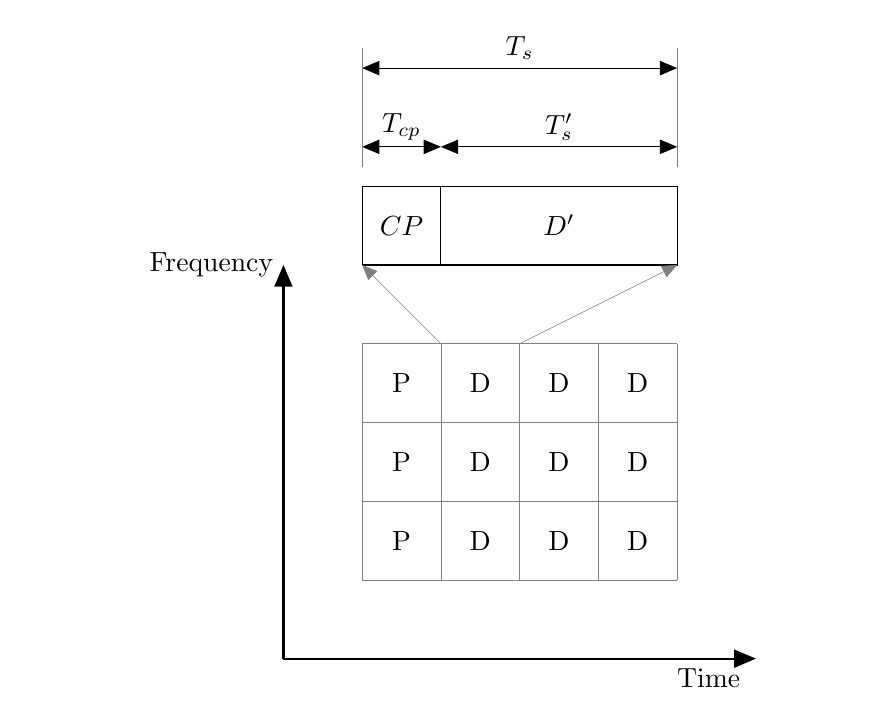
\begin{tikzpicture}[>=triangle 45,x=1.0cm,y=1.0cm]
\draw[thick,->] (0,0) -- (6,0) node [below, align=left, text width=2cm]{Time};
\draw[thick,->] (0,0) -- (0,5) node [left, align=right, text width=3cm]{Frequency};
\def\xmin{1}
\def\xminA{2}
\def\xmax{5}
\def\xmaxA{4}
\def\ymin{1}
\def\ymax{4}
\def\ymaxA{3}

\foreach \x in {\xmin,...,\xmax} {
	\draw [very thin,gray] (\x,\ymin) -- (\x,\ymax);
}
\foreach \y in {\ymin,...,\ymax} {
	\draw [very thin,gray] (\xmin,\y) -- (\xmax,\y);
}
\foreach \y in {\ymin,...,\ymaxA} {
	\draw (\xmin+0.5,\y+0.5) node {P};
}
\foreach \y in {\ymin,...,\ymaxA} {
	\foreach \x in {\xminA,...,\xmaxA} {
		\draw (\x+0.5,\y+0.5) node {D};
	}
}

\draw (1,5) -- (5,5) -- (5,6) -- (1,6) -- (1,5);
\draw (2,5) -- (2,6);
\draw [very thin,gray,->] (2,4) -- (1,5);
\draw [very thin,gray,->] (3,4) -- (5,5);
\node[align=center] at (1.5,5.5) {$CP$};
\node[align=center] at (3.5,5.5) {$D^\prime$};
\draw [<->] (1,6.5) -- (2,6.5); \draw [<->] (2,6.5) -- (5,6.5);
\node[align=center] at (1.5,6.75) {$T_{cp}$};
\node[align=center] at (3.5,6.75) {$T^\prime_s$};
\draw [<->] (1,7.5) -- (5,7.5); \node[align=center] at (3,7.75) {$T_s$};
\draw [very thin,gray] (1,6.25) -- (1,7.75);
\draw [very thin,gray] (5,6.25) -- (5,7.75);

\end{tikzpicture}

\end{center}
\end{figure}

The general design of the OFDM frame in Figure \ref{fig:ofdm_frame}.  QPSK symbols are mapped to a matrix of parallel carriers at a relatively low symbol rate in order to successfully pass through the target HF multipath channel. Pilot symbols are periodically inserted into each OFDM carrier.  At the receiver the  pilots are used to estimate the time varying phase of the channel (equalisation), and for initial acquisition (coarse frequency, and frame sync) of the received signal.  The disadvantage of pilot based schemes is they consume carrier power that would otherwise be available for the data symbols, and require the symbol rate and hence overall RF bandwidth to be increased to maintain the payload data rate.  After the IDFT stage a cyclic prefix is inserted to accommodate inter symbol interference.  The cyclic prefix also consumes carrier power and requires an increase in RF bandwidth.  The OFDM waveform details, including overheads, are explained in detail in the waveform design spreadsheet \cite{FreeDV-032}.  The \emph{Candidate 2} waveform has a RF bandwidth of approximately 1500 Hz, with 500Hz due to synchronisation overhead.

A pilot based sync system was built in PyTorch, and is used for coarse and fine timing, phase and amplitude equalisation.  Unlike classical PSK, the ML network is likely to be sensitive to amplitude variations.  Phase equalisation also allows small frequency offsets ($\pm2$ Hz) to be handled, sufficient for tests with short samples.

Several phase estimators were prototyped, and evaluated using BER measurements. Maintaining low loss synchronisation at low $E_b/N_0$ is challenging.  Using per-carrier phase estimation makes the system less dependant on fine timing accuracy and gives us the ability to handle multipath, but has higher loss than algorithms that consider all carriers at the same time.  As further work a lower latent dimension $d$ and higher $E_b/N_0$, would allocate more power to pilots, and result in less carriers.

\begin{figure}[h]
\caption{OFDM pilot based synchronisation algorithm performance, tested by measuring the BER obtained using discrete PSK symbols on an AWGN channel.  With ideal sync, the autoencoder produces intelligible speech at $E_b/N_0=-6$ dB which corresponds to BER=0.24.  Several algorithms, combined with gain and frequency offsets were simulated.}
\label{fig:ofdm_sync}
\begin{center}
\input ofdm_sync.tex
\end{center}
\end{figure}

\begin{figure}[h]
\caption{OFDM pilot based synchronisation algorithm performance, tested by measuring the BER obtained using discrete PSK symbols on an multipath (MPP) channel. The ``genie" curve is slightly better than theory, probably due to an insufficiently long run.  At the BER=0.24 threshold, the \emph{LS} algorithm has a 2dB loss compared to the ``genie" curve}
\label{fig:ofdm_sync_mp}
\begin{center}
\input ofdm_sync_mp.tex
\end{center}
\end{figure}

Figure \ref{fig:ofdm_sync} and \ref{fig:ofdm_sync_mp} plots the simulated performance of the OFDM pilot based synchronisation system on AWGN and multipath channels.  The \emph{genie} curve is the baseline rate $F_s$ OFDM system with ideal sync, and matches the theoretical BPSK BER curve.  Using this baseline system to send ML symbols, we obtain intelligible speech at $E_b/N_0=-6$, which corresponds to BER=0.24 in a digital modem.  We can use the BER=0.24 line to estimate the synchronisation loss at this operating point, which for the \emph{mean6} and \emph{LS} algorithms under realistic conditions is around 2 to 2.4 dB on AWGN, and 2dB on the  multipath channel. The \emph{LS} works better on fast fading multipath channels, so was chosen for the HF OTA trials.

Table \ref{tab:sync_losses} summarises the sync losses.  These are comparable to classical DSP OFDM data modems. Combined with $L_p$, we estimate a total sync loss of 4dB for this first pass of the ML system combined with classical pilot based synchronisation.

\begin{table} [H]
\centering
\begin{tabular}{ l | l | l}
 \hline
 Symbol & Loss (dB) & Description \\
 \hline
 $L_p$  & 0.97  & Pilot symbol overhead \\
 $L_{cp}$  & 0.97  & Cyclic prefix overhead \\
 $L_{eq}$  & 2.00  & \emph{LS} equalisation (multipath) \\
  \hline
\end{tabular}
\caption{\emph{Candidate 2} OFDM waveform design sync losses, around 4dB total.}
\label{tab:sync_losses}
\end{table}

\begin{figure}[H]
\caption{Over The Cable (OTC) VHF test. The \emph{radae} transmitter output is upsampled and shifted to 144.5 MHz using a HackRF.  The RF receive power and hence SNR is set by a step attenuator before being received by a RTL-SDR and \emph{gqrx} SDR application. Wave files recorded off air by \emph{gqrx} are presented to the \emph{radae} receiver.}
\label{fig:vhf_otc}
\begin{center}
\begin{tikzpicture}[auto, node distance=2cm,>=triangle 45,x=1.0cm,y=1.0cm,align=center,text width=1.5cm]

\node [input] (rinput) {};
\node [input, right of=rinput,node distance=0.5cm] (z) {};
\node [block, right of=z, node distance=1.5cm] (radae_tx) {\emph{radae} Tx};
\node [block, below of=radae_tx,node distance=2cm,text width=2cm] (upsampler) {Upsampler};
\node [block, below of=upsampler,node distance=2cm] (hackrf) {HackRF};
\node [block, right of=hackrf,node distance=2.5cm,text width=2cm] (attenuator) {Switched Attenuator};
\node [block, right of=attenuator,node distance=2.5cm] (rtlsdr) {RTLSDR};
\node [block, above of=rtlsdr,node distance=2cm] (gqrx) {gqrx App};
\node [block, above of=gqrx,node distance=2cm] (radae_rx) {\emph{radae} Rx};
\node [output, right of=radae_rx,node distance=2cm] (routput) {};

\draw [->] node[align=left,text width=2cm] {Input Speech} (rinput) -- (radae_tx);
\draw [->] (radae_tx) -- (upsampler);
\draw [->] (upsampler) -- (hackrf);
\draw [->] (hackrf) -- (attenuator);
\draw [->] (attenuator) -- (rtlsdr);
\draw [->] (rtlsdr) -- (gqrx);
\draw [->] (gqrx) -- node[left,text width=1cm] {\emph{.wav}} (radae_rx);
\draw [->] (radae_rx) -- (routput) node[right, align=left, text width=1.5cm] {Output Speech};

\end{tikzpicture}
\end{center}
\end{figure}

\begin{figure}[H]
\caption{Over The Cable (OTA) HF test. The \emph{radae} transmitter output is fed to the USB sound interface of a COTS HF Radio where it is shifted to HF, amplified, and transmitted over various real world HF channels to a remote KiwiSDR receiver.  Wave files recorded off air by the KiwiSDR are presented to the \emph{radae} receiver.}
\label{fig:hf_ota}
\begin{center}
\begin{tikzpicture}[auto, node distance=2cm,>=triangle 45,x=1.0cm,y=1.0cm,align=center,text width=1.5cm]

\node [input] (rinput) {};
\node [input, right of=rinput,node distance=0.5cm] (z) {};
\node [block, right of=z, node distance=1.5cm] (radae_tx) {\emph{radae} Tx};
\node [block, below of=radae_tx,node distance=2cm] (hf_tx) {HF Radio};
\node [block, right of=hf_tx,node distance=2.5cm] (hf_channel) {HF Channel};
\node [block, right of=hf_channel,node distance=2.5cm] (kiwisdr) {KiwiSDR};
\node [block, above of=kiwisdr,node distance=2cm] (radae_rx) {\emph{radae} Rx};
\node [output, right of=radae_rx,node distance=2cm] (routput) {};

\draw [->] node[align=left,text width=2cm] {Input Speech} (rinput) -- (radae_tx);
\draw [->] (radae_tx) -- (hf_tx);
\draw [->] (hf_tx) -- (hf_channel);
\draw [->] (hf_channel) -- (kiwisdr);
\draw [->] (kiwisdr) -- node[left,text width=1cm] {\emph{.wav}} (radae_rx);
\draw [->] (radae_rx) -- (routput) node[right, align=left, text width=1.5cm] {Output Speech};

\end{tikzpicture}
\end{center}
\end{figure}

\subsection{March 2024 Results}

In March 2024, the system was tested over a VHF OTC AWGN path and OTA on a variety of real world Australian HF multipath paths. Figure \ref{fig:vhf_otc} and Figure \ref{fig:vhf_otc} describe the experimental configurations.  Wave files containing a sine wave tone, compressed SSB, and the \emph{radae} signal were sent over the same channel at the same time. The speech quality obtained was consistent with the simulations and competitive with SSB sent over the same channel at the same time.

Take aways:
\begin{enumerate}
\item We have combined ML vocoder, ML autoencoder and classical DSP OFDM to build a system capable of sending speech over radio channels.  It is robust to AWGN and multipath channel impairments.  Our initial simulation, VHF OTC, and HF OTA tests suggest performance competitive with the analog SSB at the same $C/N_0$.
\item The total ``sync losses" due to pilot, cyclic prefix overheads and non-ideal equalisation are around 4dB.  It is conceivable these can be reduced using ML rather than classical DSP. 
\item The ML algorithms run at a 40ms frame rate (with some DSP at the OFDM 20ms symbol rate), resulting in modest CPU requirements.  The PyTorch simulation code runs several times faster than real time in inference mode.
\item Simulation and initial HF OTA results show surprisingly good performance on multipath channels where the period of the fading (100's of ms) is large compared to the 40ms analysis window of the ML code.  Classical DSP would require a 1000-2000 ms interleaver (introducing a algorithmic delay of the same order) for similar robustness to fading on these channels.
\item Unlike regular PSK, we require magnitude estimation and correction, due to the limited dynamic range of ML systems and the wide dynamic range of radio signals.
\item The \emph{Candidate 2} OFDM frame design \cite{FreeDV-032} contains three latent vectors $z$, so introduces an algorithmic delay of 120ms, due to OFDM framing considerations.  This is tolerable in a PTT radio system, but ideally should be reduced.
\item Substituting classical PSK digital symbols and measuring BER is a very useful way to test sync, and to allows us to verity $E_b/N_0$ using BER measurements during development.
\item Much of our development effort to date has concerned with the ``is this too good to be true" question; to date significantly more effort was put into noise calibration, synchronisation algorithms and testing than the actual ML.
\end{enumerate}

Further work:
\begin{enumerate}
\item Try a low dimension latent vector, e.g. $d=40$, and see if similar speech quality can be obtained at 3dB higher $E_b/N_0$. This would result in lower sync losses and RF bandwidth for the same channel SNR or $C/N_0$, as the $E_b/N_0$ of the pilots would be increased. Does the encoder output still resemble BPSK, or is it training to a higher order constellation?
\item There is significant synchronisation loss from the classical DSP OFDM waveform and associated sync algorithms. Attempt to use the ML network to perform frequency, phase and amplitude equalisation, with or without passing the pilots to the decoder.  An initial attempt (model07) without pilots showed some ability to correct phase, frequency, and magnitude offsets, but resulted in some performance degradation. However this may be acceptable if comparable to the pilot based sync losses. Some pilot or unique word injection may still be required to perform coarse and fine timing estimation using classical DSP running at the sample rate.
\item We may be able to improve on algorithmic delay using ML sync techniques that are less dependant on traditional OFDM framing considerations.
\item Some form or interleaving, or a long time window for the ML network, may improve performance.
\item Work to improve the current classical DSP sync, e.g. from Figure \ref{fig:ofdm_sync} a feedback loop to track out frequency offsets is worth 1 dB.
\item Include PAPR optimisation and rate $F_s$ multipath channels in the training.
\item To better model SSB, locate a better analog compressor, a 3rd party reference implementation in software form would be useful.
\item Definition of lower limit link closure for this use case, for example ``CQ CQ, and callsign, enough to produce a QSO report".
\item For a practical implementation, coarse amplitude and timing need to be updated regularly. As we are testing short samples, a single block estimate is used at present.
\end{enumerate}

\section{Comparison with Other Speech Waveforms}

We wish to compare the potential of our radio autoencoder with existing waveforms used for speech transmission over radio channels.  This section assumes the \emph{radae} system can send intelligible speech at an $E_b/N_0$ of -6dB, with a PAPR of 1dB, both results have been demonstrated in simulation (but not at the time of writing together over real world radio channels).  We include a 3dB synchronisation overhead, anticipating modest improvements over the 4dB obtained with our proof of concept system described above.

We start with the assumption that we have a transmitter of $C$ watts, and an AWGN channel with a spectral noise density of $N_0$ watts/Hz. As the speech waveforms being considered vary in bandwidth we will choose $C/N_0$ as the SNR metric.

The $C/N_0$ (in dBHz) at the demodulator input of a terrestrial radio receiver is given by:
\begin{equation}
\frac{C}{N_0} = P - PAPR - L_{path} - NF + 174
\end{equation}
where $P$ is the maximum output power of the transmitter power amplifier, $PAPR$ is the Peak to Average Power Ratio of the waveform, $L_{path}$ is the path loss, $NF$ is the noise figure of the receiver.  For example consider a 400 MHz FM hand held radio over a 1km urban (non line of site) path.  The radio has a 1W (30 dBm) power output, $L_{path}=120$ dB, with noise dominated by ambient EMI such that $NF=10$ dB. $C/N_0 = 30 - 0 - 120 - 10 + 174 = 74$ dBHz, sufficient for good quality speech (Table \ref{tab:waveforms_good}).

Note that $C/N_0$ at the demodulator is a function of the waveform PAPR.  With all other link properties (e.g. peak PA power, noise figure, path loss) being equal, a high PAPR reduces the $C/N_0$ available at the receiver.  We effectively ``back off" the transmitter power from the maximum $P$ by the PAPR.  We assume the PA is capable of sustaining $P$ watts indefinitely, i.e. it is only the waveform choice that lowers the average power. As PAPR varies by waveform and has an impact on the $C/N_0$ available the receiver, it should be included in any metric for comparison of waveforms.  We define $P/N_0$ as:
\begin{equation}
P/N_0 = C/N_0 + PAPR
\end{equation} 
A waveform that delivers intelligible speech at a low $P/N_0$ is the target.  A low PAPR waveform has other desirable properties, such as greater PA efficiency, longer battery life, and the use of low cost semiconductors in the radio power amplifier electronics.

\begin{table} [H]
\centering
\begin{tabular}{  m{3.5cm} | m{7cm}  }
 \hline
 Waveform             & Threshold \\
 \hline
 Single Sideband      & 0dB SNR in 3000Hz noise BW, 2400Hz audio bandwidth, Tx speech compressor with 6dB PAPR \\
 Frequency Modulation & -120 dBm quoted for many NBFM radios, 54dB above -174dBm/Hz noise floor \\
 FreeDV 700D          & 10\% PER threshold at -2dB SNR in 3000Hz noise BW \\
 Radio Autoencoder    & Intelligible speech at $E_b/N_0=-6$ dB, $R_b=2000$ symbols/s, 3dB sync overhead, a PAPR of 1dB \\
 \hline
\end{tabular}
\caption{Thresholds for speech link closure for each waveform. The link is considered closed when the speech is barely intelligible to a trained listener.}
\label{tab:waveforms_thresh}
\end{table}

TODO: include 1st gen VHF/UHF digital voice - I think they go down to -123 dB (5\%) BER, but speech quality is sub FM.

\begin{table} [H]
\centering
\begin{tabular}{  m{3.5cm} | m{7cm}  }
 \hline
 Waveform             & Threshold $C/N_0$ calculations (dBHz) \\
 \hline
 Single Sideband      & $0 + 10log_{10}(3000) = 35$ \\
 Frequency Modulation & $-120 + 174 = 54$ \\
 FreeDV 700D          & $-2 + 10log_{10}(3000) = 33$ \\
 Radio Autoencoder    & $-6 + 10log_{10}(2000) + 3 = 30$ \\
 \hline
\end{tabular}
\caption{Threshold $C/N_0$ calculations.}
\label{tab:waveforms_thresh_calc}
\end{table}

\begin{table} [H]
\centering
\begin{tabular}{l l r r r r r}
 \hline
 Waveform             & Abbr  & RF BW & PAPR & $C/N_0$ & $P/N_0$ & $\Delta$ \\
 \hline
 Single Sideband      & SSB   & 2400  &  6 & 35 & 41 & -10 \\
 Frequency Modulation & NBFM  & 16000 &  0 & 54 & 54 & -23 \\
 FreeDV 700D          & 700D  & 1100  &  4 & 33 & 37 & -6  \\
 Radio Autoencoder    & radAE & 1400  &  1 & 30 & 31 &  0  \\
 \hline
\end{tabular}
\caption{Comparison of link closure by waveform over AWGN channels. A lower $P/N_0$ is better.}
\label{tab:waveforms_linkclosure}
\end{table}

\begin{table} [H]
\centering
\begin{tabular}{l r r r r}
 \hline
 Waveform             & Audio BW & $C/N_0$ & $P/N_0$ & $\Delta$ \\
 \hline
 Radio Autoencoder    & 8000 & 36 & 37 &   0 \\
 Frequency Modulation & 3000 & 64 & 64 & -27 \\
 Single Sideband      & 3000 & 55 & 61 & -24 \\
 \hline
\end{tabular}
\caption{Comparison of good quality ``arm chair copy" by waveform over AWGN channels. They are ranked in terms of maximum achievable speech quality. FreeDV 700D has been omitted because of its low speech quality even at high SNR. Even at 20dB SNR there is noticeable noise in received SSB, although DSP based noise reduction may help. Only the radio autoencoder delivers wideband (8000 Hz) speech.}
\label{tab:waveforms_good}
\end{table}

\section{CPU and Memory Requirements}

\begin{table} [H]
\centering
\begin{tabular}{l l l}
 \hline
 Module & MMACS & Memory (kbyte) \\
 \hline
 Feature Extraction &  - & - \\
 RADAE Encoder & 80 & 1000 \\
 OFDM Tx & - &  - \\
 \hline
 Totals & 80 & 1000 \\
 \hline
\end{tabular}
\caption{Estimates of RADAE transmitter (Tx) CPU and Memory Requirements.}
\label{tab:radae_tx_resources}

\end{table}
\begin{table} [H]
\centering
\begin{tabular}{l l l}
 \hline
 Module & MMACS & Memory (kbyte) \\
 \hline
 FARGAN vocoder &  300/175 &  800 \\
 RADAE Decoder & 80 & 1000 \\
 OFDM Rx & - & - \\
 \hline
 Totals & 380/255 & 1800 \\
 \hline
\end{tabular}
\caption{Estimates of RADAE receiver (Rx) CPU and Memory Requirements.}
\label{tab:radae_rx_resources}
\end{table}

Tables \ref{tab:radae_tx_resources} and \ref{tab:radae_rx_resources} contain estimates of the CPU and memory resources. Typical PTT radio uses-case are half duplex, so the Tx and Rx would not be required to run at the same time.  The receiver dominates, due to the FARGAN vocoder. MMACS is the number 8-bit multiply and accumulates per second divided by 1E6. The memory is mainly ML weights which are read-only.  However memory access needs to be fast to maintain the MMAC rate - each MMAC is assumed to include any required loads. A non-SIMD floating point implementation (where multiple and accumulate are separate operations) would take twice the number of operations when measured in MFLOPS, and four times the memory.
 
The FARGAN author recommends a 64-bit ARM with NEON extensions as a minimum machine (Cortex-M is likely too small). The current FARGAN vocoder requires 300 MMACs, a slightly lower quality version is available that uses 175 MMACS.  The classical DSP Feature Extraction uses comparatively small amounts of CPU and memory, but currently requires floating point hardware.

The RADAE ML CPU hasn't been measured accurately but runs in real time in Python, and is less than the FARGAN decoder (i.e. the FARGAN vocoder dominates the CPU).  For an initial estimate we have approximated the RADAE CPU as 25\% of FARGAN. The RADAE encoder and decoder require approximately the same CPU, and similar memory (ML weights).  It may be possible to reduce the number of weights and CPU, as the optimal size of the RADAE network has not been studied.

The classical DSP OFDM processing requires less resources but hasn't been accurately measured at this time.  Comparable modems at similar symbol rates run on a fraction of Cortex-M micro-controllers. Unlike the ML modules, it currently requires floating point hardware.  For a first approximation we assume OFDM resource requirements are small compared to the ML modules.

\section{Training for low PAPR}

To train for low PAPR we constrain the magnitude of the complex rate $F_s$ time domain transmit signal $|x(n)| \le 1$.  We wish to train for a range of SNRs so require an expression to compute $\sigma$ for a given target $E_b/N_0$.

Consider a hybrid ML-DSP system where we constrain $|x(n)|$ in the time domain, but perform all other processing at rate $R_s$ in the frequency domain using classical DSP OFDM techniques.  After the bottleneck is applied to $x(n)$, we DFT to transform back to the frequency domain, apply a magnitude only multipath model, than add AWGN noise to simulate the received frequency domain symbols $\hat{q}$.

Given this model, we wish to inject calibrated AWGN noise. Consider one time domain OFDM carrier $x(n)$ with magnitude $B$. We take the length $M$ DFT to determine the magnitude $A_q$ of the corresponding frequency domain PSK symbol:
\begin{equation}
\begin{split}
x(n) &= Be^{j(2 \pi n k/M + \theta)} \\
X(k) &= \sum_{n=0}^{M-1} x(n) e^{-j(2 \pi n k/M)} \\
     &= BMe^{j\theta} \\
|X(k)| &= A_q = BM
\end{split}
\end{equation}

We have $N_c$ carriers, and the bottleneck constrains the total time domain power of all carriers to be approximately 1:
\begin{equation}
\begin{split}
N_cB^2 &= 1 \\
B        &= \frac{1}{\sqrt{N_c}}
\end{split}
\end{equation}
Using (\ref{eq:Eb_Es}) and (\ref{eq:noise_sigma}) we can find an expression for $\sigma$ given $E_b/N_0$:
\begin{equation}
\begin{split}
\sigma &= \frac{A_b}{\sqrt{E_b/N_0}} \\
\sigma &= \frac{A_q}{\sqrt{2 E_b/N_0}} \\
\sigma &= \frac{M}{\sqrt{2 N_c E_b/N_0}} 
\end{split}
\end{equation}
The factor of $\sqrt{2}$ on the denominator accounts for $A_q$ being the amplitude of a PSK symbol, whereas (\ref{eq:noise_sigma}) is configured for BPSK symbols. For example if $A_b=1$, $A_q=\sqrt{2}$.
\section{Glossary}

\begin{table} [H]
\centering
\begin{tabular}{l l l}
 \hline
 Symbol & Explanation & Units \\
 \hline
 $B$ & noise or signal bandwidth & Hz \\
 $C$ & Carrier (transmitter) power $C=S$ for this study \\
 $C/N_0$ & Carrier power/spectral noise density \\
 $d$ & dimension of latent vector $\bf{z}$ \\
 $E_b/N_0$ & energy per BPSK symbol on spectral noise density \\
 $E_q/N_0$ & energy per QPSK symbol on spectral noise density \\
 $N$ & total noise power & Watts \\
 $N_c$ & Number of carriers  \\
 $N_0$ & Noise power in 1 Hz of bandwidth  \\
 $P/N_0$ & Peak transmitter power/spectral noise density \\
 $\bf{q}$ & vector of QPSK symbols \\ 
 $q_i$ & single QPSK symbol, element of $\bf{q}$ \\ 
 $R_b$ & BPSK symbol rate & symbols/second \\
 $R_q$ & QPSK symbol rate & symbols/second \\
 $R_s$ & OFDM per carrier QPSK symbol rate & symbols/second \\
 $R_z$ & latent vector update rate & Hz \\
 $SNR$ & signal to noise Ratio \\
 $S$ & total signal (carrier) power & Watts \\
 $T_b$ & BPSK symbol period & seconds \\
 $T_q$ & QPSK symbol period & seconds \\
 $T_s$ & OFDM per carrier QPSK symbol period & seconds\\
 $T_z$ & time between latent vector updates & seconds\\
 $r_i$ & noise sample \\
 $\bf{z}$ & Autoencoder output latent vector \\ 
 $z_i$ & single latent vector element of $\bf{z}$, a BPSK symbol \\ 
 \hline
\end{tabular}
\caption{Glossary of Symbols}
\end{table}

\nocite{*}
\bibliographystyle{plain}
\bibliography{radae_refs}
\end{document}


\end{document}
